\documentclass[11pt]{book}

%%%%%%%%%%%%%%Include Packages%%%%%%%%%%%%%%%%%%%%%%%%%%
\usepackage{xcolor}
\usepackage{mathtools}
\usepackage[a4paper, total={6in, 8in}, margin=1in]{geometry}
\usepackage{amsmath}
\usepackage{amssymb}
\usepackage{paralist}
\usepackage{rsfso}
\usepackage{amsthm}
\usepackage{wasysym}
\usepackage[inline]{enumitem}   
\usepackage{hyperref}
\usepackage{tocloft}
\usepackage{wrapfig}
\usepackage{titlesec}
\usepackage{colortbl}
\usepackage{stackengine} 
\usepackage{csvsimple}
\usepackage{listings}
%%%%%%%%%%%%%%%%%%%%%%%%%%%%%%%%%%%%%%%%%%%%%%%%%%%%%%%%



%%%%%%%%%%%%%%%Code%%%%%%%%%%%%%%%%%%%%%%%%%%%%%%%%%%%%%
\definecolor{codegreen}{rgb}{0,0.6,0}
\definecolor{codegray}{rgb}{0.5,0.5,0.5}
\definecolor{codepurple}{rgb}{0.58,0,0.82}
\definecolor{backcolour}{rgb}{0.95,0.95,0.92}

\lstdefinestyle{mystyle}{
    backgroundcolor=\color{backcolour},   
    commentstyle=\color{codegreen},
    keywordstyle=\color{magenta},
    numberstyle=\tiny\color{codegray},
    stringstyle=\color{codepurple},
    basicstyle=\ttfamily\footnotesize,
    breakatwhitespace=false,         
    breaklines=true,                 
    captionpos=b,                    
    keepspaces=true,                 
    numbers=left,                    
    numbersep=5pt,                  
    showspaces=false,                
    showstringspaces=false,
    showtabs=false,                  
    tabsize=2
}
%%%%%%%%%%%%%%%%%%%%%%%%%%%%%%%%%%%%%%%%%%%%%%%%%%%%%%%%




%%%%%%%%%%%%%%%Chapter Setting%%%%%%%%%%%%%%%%%%%%%%%%%%
\definecolor{gray75}{gray}{0.75}
\newcommand{\hsp}{\hspace{20pt}}
\titleformat{\chapter}[hang]{\Huge\bfseries}{\thechapter\hsp\textcolor{gray75}{$\mid$}\hsp}{0pt}{\Huge\bfseries}
%%%%%%%%%%%%%%%%%%%%%%%%%%%%%%%%%%%%%%%%%%%%%%%%%%%%%%%%

%%%%%%%%%%%%%%%%%Theorem environments%%%%%%%%%%%%%%%%%%%
\newtheoremstyle{break}
  {\topsep}{\topsep}%
  {\itshape}{}%
  {\bfseries}{}%
  {\newline}{}%
\theoremstyle{break}
\theoremstyle{break}
\newtheorem{axiom}{Axiom}
\newtheorem{thm}{Theorem}[section]
\renewcommand{\thethm}{\arabic{section}.\arabic{thm}}
\newtheorem{lem}{Lemma}[thm]
\newtheorem{prop}[lem]{Proposition}
\newtheorem{corL}{Corollary}[lem]
\newtheorem{corT}[lem]{Corollary}
\newtheorem{defn}{Definition}[corL]
\newenvironment{indEnv}[1][Proof]
  {\proof[#1]\leftskip=1cm\rightskip=1cm}
  {\endproof}
%%%%%%%%%%%%%%%%%%%%%%%%%%%%%%%%%%%%%%%%%%%%%%%%%%%%%%


%%%%%%%%%%%%%%%%%%%%%%%Integral%%%%%%%%%%%%%%%%%%%%%%%
\def\upint{\mathchoice%
    {\mkern13mu\overline{\vphantom{\intop}\mkern7mu}\mkern-20mu}%
    {\mkern7mu\overline{\vphantom{\intop}\mkern7mu}\mkern-14mu}%
    {\mkern7mu\overline{\vphantom{\intop}\mkern7mu}\mkern-14mu}%
    {\mkern7mu\overline{\vphantom{\intop}\mkern7mu}\mkern-14mu}%
  \int}
\def\lowint{\mkern3mu\underline{\vphantom{\intop}\mkern7mu}\mkern-10mu\int}
%%%%%%%%%%%%%%%%%%%%%%%%%%%%%%%%%%%%%%%%%%%%%%%%%%%%%%



\newcommand{\R}{\mathbb{R}}
\newcommand{\N}{\mathbb{N}}
\newcommand{\Z}{\mathbb{Z}}
\newcommand{\Q}{\mathbb{Q}}
\newcommand{\C}{\mathbb{C}}
\newcommand{\T}{\mathcal{T}}
\newcommand{\M}{\mathcal{M}}
\newcommand{\Symm}{\text{Symm}}
\newcommand{\Alt}{\text{Alt}}
\newcommand{\Int}{\text{Int}}
\newcommand{\Bd}{\text{Bd}}
\newcommand{\Power}{\mathcal{P}}
\newcommand{\ee}[1]{\cdot 10^{#1}}
\newcommand{\spa}{\text{span}}
\newcommand{\sgn}{\text{sgn}}
\newcommand{\degr}{\text{deg}}
\newcommand{\pd}{\partial}
\newcommand{\that}[1]{\widetilde{#1}}
\newcommand{\lr}[1]{\left(#1\right)}
\newcommand{\vmat}[1]{\begin{vmatrix} #1 \end{vmatrix}}
\newcommand{\bmat}[1]{\begin{bmatrix} #1 \end{bmatrix}}
\newcommand{\pmat}[1]{\begin{pmatrix} #1 \end{pmatrix}}
\newcommand{\rref}{\xrightarrow{\text{row\ reduce}}}
\newcommand{\txtarrow}[1]{\xrightarrow{\text{#1}}}
\newcommand\oast{\stackMath\mathbin{\stackinset{c}{0ex}{c}{0ex}{\ast}{\Circle}}}


\newcommand{\note}{\color{red}Note: \color{black}}
\newcommand{\remark}{\color{blue}Remark: \color{black}}
\newcommand{\example}{\color{green}Example: \color{black}}
\newcommand{\exercise}{\color{green}Exercise: \color{black}}

%%%%%%%%%%%%%%%%%%%%%%Roman Number%%%%%%%%%%%%%%%%%%%%%%%
\makeatletter
\newcommand*{\rom}[1]{\expandafter\@slowromancap\romannumeral #1@}
\makeatother
%%%%%%%%%%%%%%%%%%%%%%%%%%%%%%%%%%%%%%%%%%%%%%%%%%%%%%%%%

%%%%%%%%%%%%table of contents%%%%%%%%%%%%%%%%%%%%%%%%%%%%
\setlength{\cftchapindent}{0em}
\cftsetindents{section}{2em}{3em}

\renewcommand\cfttoctitlefont{\hfill\huge\bfseries}
\renewcommand\cftaftertoctitle{\hfill\mbox{}}

\setcounter{tocdepth}{2}
%%%%%%%%%%%%%%%%%%%%%%%%%%%%%%%%%%%%%%%%%%%%%%%%%%%%%%%%%


%%%%%%%%%%%%%%%%%%%%%Footnotes%%%%%%%%%%%%%%%%%%%%%%%%%%%
\newcommand\blfootnote[1]{%
  \begingroup
  \renewcommand\thefootnote{}\footnote{#1}%
  \addtocounter{footnote}{-1}%
  \endgroup
}
%%%%%%%%%%%%%%%%%%%%%%%%%%%%%%%%%%%%%%%%%%%%%%%%%%%%%%%%%

%%%%%%%%%%%%%%%%%%%%%Section%%%%%%%%%%%%%%%%%%%%%%%%%%%%%
\makeatletter
\def\@seccntformat#1{%
  \expandafter\ifx\csname c@#1\endcsname\c@section\else
  \csname the#1\endcsname\quad
  \fi}
\makeatother
%%%%%%%%%%%%%%%%%%%%%%%%%%%%%%%%%%%%%%%%%%%%%%%%%%%%%%%%%

%%%%%%%%%%%%%%%%%%%%%%%%%%%%%%%%%%%Enumerate%%%%%%%%%%%%%%
\makeatletter
% This command ignores the optional argument 
% for itemize and enumerate lists
\newcommand{\inlineitem}[1][]{%
\ifnum\enit@type=\tw@
    {\descriptionlabel{#1}}
  \hspace{\labelsep}%
\else
  \ifnum\enit@type=\z@
       \refstepcounter{\@listctr}\fi
    \quad\@itemlabel\hspace{\labelsep}%
\fi}
\makeatother
\parindent=0pt
%%%%%%%%%%%%%%%%%%%%%%%%%%%%%%%%%%%%%%%%%%%%%%%%%%%%%%%%%%


\begin{document}

	\begin{titlepage}
		\begin{center}
			\vspace*{1cm}
			\Huge \color{red}
				\textbf{Lab 10 Report}\\
			\vspace{0.5cm}			
			\Large \color{black}
				Math 391 - Introduction to Modern Physics Lab\\
				Professor Wayne Lau\\	
				University of Michigan\\
			\vspace{3cm}

			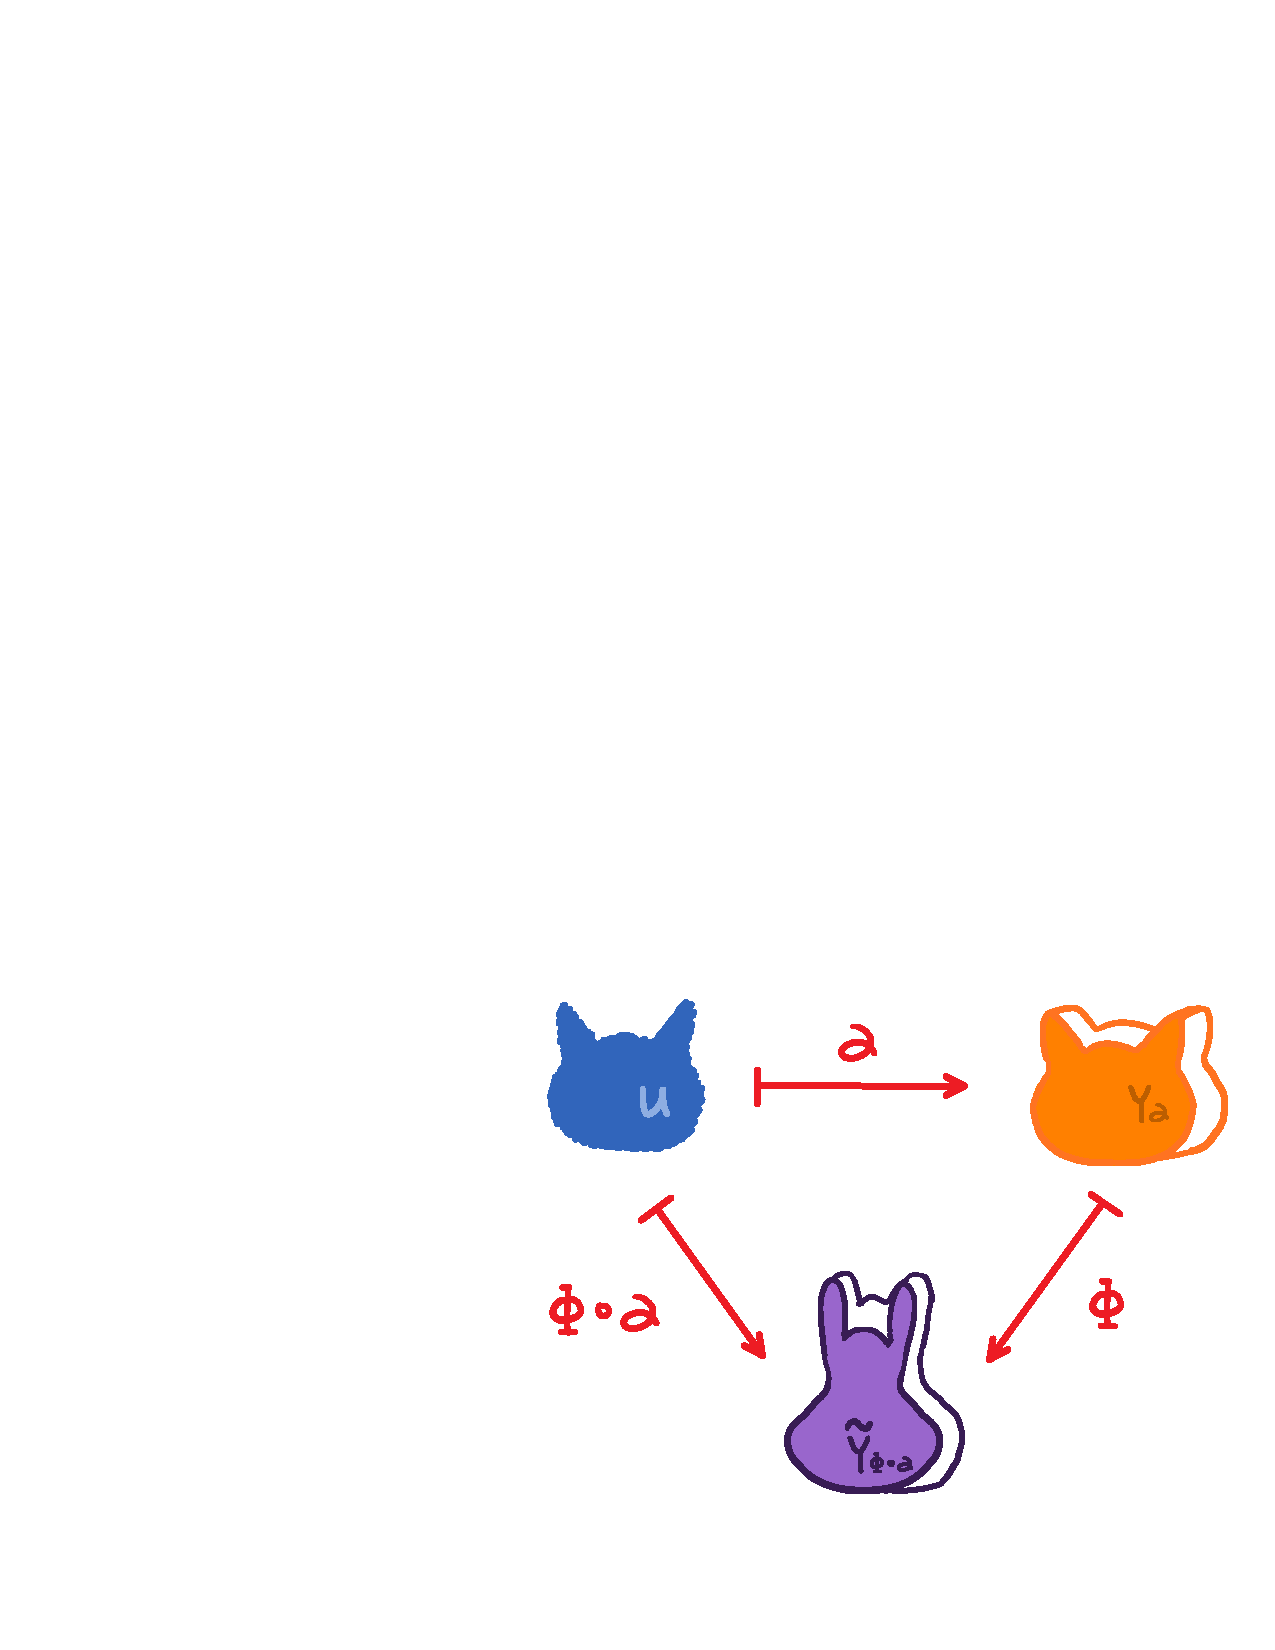
\includegraphics[scale=0.6]{Intkform1.pdf}\\
			\hfill\break
			\color{gray}Figure 0. Integrating k-form over a manifold\\is independent on the use of coordinate patches\color{black}
			
			
			
			\vspace{5cm}
			\LARGE
				\textbf{Jinyan Miao}\\
				\hfill\break
				\LARGE Fall 2022\\
			\vspace{1cm}

		\vspace*{\fill}
		\end{center}			
	\end{titlepage}


\newpage
\tableofcontents
\addtocontents{toc}{~\hfill\textbf{Page}\par}


\chapter*{Lab 10 - The Hall Effect \\and Conductivity of 
Semiconductors}
\setcounter{chapter}{10}
\section{Introduction}
The phenomenon of Hall effect was discovered by Edvin H. Hall in 1879. A charge $q$, moving at a velocity $\vec{v}$, perpendicular a magnetic field $\vec{B}$, with experience a force $\vec{F} = q \vec{v}\times \vec{B}$. If a conducting  material in a magnetic field has physical bounds restricting such motion, the accumulated displaced charge will create a net vertical electric field, and such phenomenon is called the Hall effect, and the resulting Hall electric field is given by the following:
\begin{align}
\vec{E}_H = -\frac{1}{nq}\vec{J}\times \vec{B}\qquad\qquad \text{where }\vec{J} = nq\vec{v}
\end{align}
where $n$ is the charge carrier density.\\

In real materials, the translational  symmetry of the crystal lattice   imposes energy band gaps when the periodicity of the electronic wave function is commensurate 
with the lattice spacing. For semiconducting materials, the energy gap between the valence band and the conduction band, denoted as $E_g$, is of order $1\, eV$. Thermal excitations will promote valence electrons into the conduction band to population densities given by:
\begin{align}
n_c = n_v e^{-E_g /2kT}
\end{align}
where $n_v$ and $n_c$ are the valence and conduction band carrier densities. However, for most applications, the doping levels of the semiconductors are high enough that at room temperature the conductivity of the material is dominated by the
extrinsic carriers due to the doping process and not the thermal excitations common to intrinsic samples.\footnote{Akerlof, Carl W., \textit{Physics 391 Experiment 10 Lab Manual}, (2018)} In Lab 10 of Physics 391, we  explore  the  electrical  properties  of  crystalline  germanium  by varying the temperature, the immersion in a magnetic field, and the applied voltage across the material. 


\section{Experimental Setup}
In this lab, we explore the electronic behavior of a lightly $p$-doped germanium crystal by measuring the Hall voltage and the conductivity as a function of temperature. The magnetic field in this experiment is supplied by the array of permanent rare earth magnets of magnitude approximately $1\, T$. The direction of the magnetic field is determined by knowing the force experienced by a charged wire placed in the supplied field. The magnetic field in the apparatus is found to be oriented counterclockwise. We first verify that the Hall voltage is well described by (10.2). The germanium sample is inserted in the magnet ring and the temperature is assumed to be close to $20^\circ C$. As we change the current through the sample from $-60\, mA$ to $60\, mA$, the Hall voltage is measured using a multimeter, and the voltage across the sample is also measured using another multimeter. The crystal cross sectional are is $1\, mm \times 10\, mm = 10^{-5}\, m^2$. The sample width is $10\, mm$. \\

We also check the Hall voltage response over the change of magnetic field strength by lifting the germanium sample to about half inside the magnet gap, we observe that the corresponding change in the magnetic field density is about half of the original value.\\

Then we explore the effects on the Hall voltage when germanium crystal temperature is varied. The current through the sample in this part is fixed at $60\, mA$. The orientation of the B field is set to be inward (details about the effect of the orientation of the B field is discussed in section 10.3.1). The sample temperature is first raised up to $140^\circ C$. Then we let the sample cool down by itself and at the same time we measure the Hall voltage and the voltage across the sample. Measurements are taken until the sample reaches around $30^\circ C$, a bit above the room temperature. The intervals between measurements in this part is every $10^\circ C$ drop in temperature.\\

\section{Data Analysis}
\subsection{Current Dependence}
In this part, we will present the result of Hall voltage's dependence on the current through the $p$-doped germanium crystal sample. 
\begin{center}
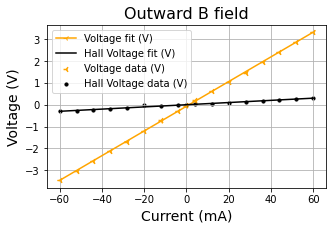
\includegraphics[scale=0.6]{1}
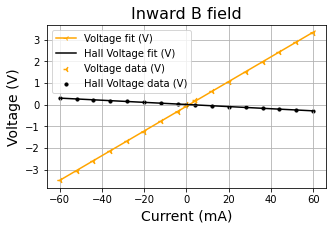
\includegraphics[scale=0.6]{2}
\end{center}
We have performed the measurement twice, with opposite orientation of the magnetic field, one is labeled as \textit{Outward B field} and the other is labeled as \textit{Inward B field}. The linear regression parameters are given by the followings:
\begin{center}
\begin{tabular}{|c|c|c|c|c|}
\hline
Orientation of B field & slope $k$ & st. dev. of $k$ ($\sigma_k$) & $y$-intercept $b$ & st. dev. of $b$ ($\sigma_b$)\\
\hline
Outward &  0.005023 & 0.000164 & -0.000406 & 0.005884\\
\hline
Inward & -0.004900 & 0.000200 & 0.005065 & 0.000732\\
\hline
\end{tabular}\\
\hfill\break
\textbf{Table 1. Hall Voltage Linear Regression Parameters}


\hfill\break
\hfill\break
\begin{tabular}{|c|c|c|c|c|}
\hline
Orientation of B field & slope $k$ & st. dev. of $k$ ($\sigma_k$) & $y$-intercept $b$ & st. dev. of $b$ ($\sigma_b$)\\
\hline
Outward &  0.056681 & 0.000194 & -0.070612 & 0.006933\\
\hline
Inward & 0.057014 & 0.000264 & -0.077259 & 0.009445\\
\hline
\end{tabular}\\
\hfill\break
\textbf{Table 2. Voltage Across Sample Linear Regression Parameters}
\end{center}
To investigate the relationship between Hall voltage and current, Table 1 is the one that we are interested in. For the outward B field orientation, the $r^2$-value for the linear regression is $0.9841714$, and for the inward B field orientation, the $r^2$-value for the linear regression is $0.9997386$. These results statistically indicate that we have a linear relationship between the Hall voltage and the current. This verifies the linear relationship between the Hall voltage $V_H = E_H \cdot w$ and current $|\vec{J}|$ through the sample as predicted by (10.1). Here $w$ denotes the width of the sample. Moreover, we expect there is no difference between the absolute value of the linear dependence coefficients in the linear regression for the two orientations of the B field. That is, we should have: $$|k_{\text{inward B}}| = |k_{\text{outward B}}|$$
Here we simply note that $|k_{\text{outward B}}|$ is captured within $1$-$\sigma_{k_{\text{inward B}}}$, and $|k_{\text{inward B}}|$ is captured within $1$-$\sigma_{k_{\text{outward B}}}$. This should suffice to show statistically that the absolute value of the slopes are equal. Hence we can conclude that the orientation of the magnetic field only affects the direction of the Hall electric field, and hence the sign of the Hall voltage, and it does not affect the magnitude of the Hall electric field and Hall voltage. Moreover, based on the set up configuration and the sign of the Hall voltage $V_H$, we conclude here the charge carriers in the sample are of positive sign, that is, they are holes instead of electrons. \\

\subsection{Temperature Dependence and Energy Gap}
For this part of the experiment, the current through the sample is fixed at $60\, mA$, and the orientation of the B field is inward. First we present the data of Hall voltage over the temperature of the sample:
\begin{center}
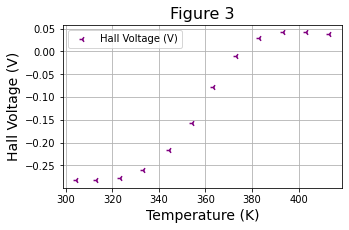
\includegraphics[scale=0.6]{3}
\end{center}
From Fig. 3, we observe that the Hall voltage changes sign as temperature increases to around $380\, K$. Here we estimate the germanium band gap potential $E_g$. First we compute the conductivity of the sample, and obtain the following figure:
\begin{center}
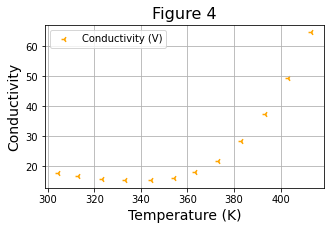
\includegraphics[scale=0.6]{4}
\end{center}
Note that, according to the Physics 391 Lab Manual, the conductivity is defined by the ratio of the current density to the applied electric field which in turn is the longitudinal  voltage applied across the sample  divided by the length of 20 mm. In  the high temperature regime, the conductivity is dominated by electrons promoted into the conduction band as 
described  by (10.2), while  close  to  room  temperature,  the  conductivity  is  modulated  by  electron-
phonon collisions that disrupt electron motion. These two effects can be modeled by the following:
\begin{align}
\sigma(T) = a+\frac{b}{T}+ce^{-eE_g/2kT}
\end{align}
where $a,b,c,E_g$ are constants. We fit (10.3) using our data and obtain the following:
\begin{center}
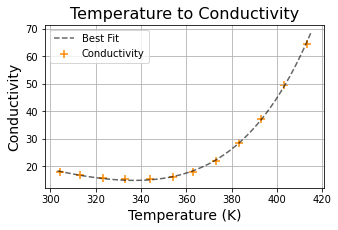
\includegraphics[scale=0.6]{5}
\end{center}
The parameters of the fit is given by the followings:
\begin{center}
\begin{tabular}{|c|c|c|}
\hline
Parameter & value & st. dev.\\
\hline
a& -49.1184 & 7.7010 \\
\hline
b & 20247.5686 & 2370.6199\\
\hline
c & 15807680.0778 & 7508472.5915 \\
\hline
$E_g$& 0.8829 & 0.03567\\
\hline
\end{tabular}
\end{center}
Here we see that $E_g = 0.8829 \pm 0.03567\, V$. While the standard accepted value for $E_g$ is $0.67\, V$, we see here our the standard value is not captured within $3$-$\sigma$ of our experimental value of $E_g$, that is we have $0.67 - 0.88 > 3\sigma = 3\cdot 0.04 = 0.12$. Hence we conclude that the standard accepted value for $E_g$ is not statistically well-predicted by our data.\\


From (10.1), we can estimate the density of carriers at room temperature in the germanium sample, where we use $V_H/I \approx 0.005\cdot 10^{3}$ as we have estimated in 10.3.1. 
\begin{align*}
n = \frac{JB}{E_Hq} = \frac{IBw}{AV_Hq}=\frac{Bw}{Aq}\frac{I}{V_H} = \frac{(1\,T)(10\cdot 10^{-3}\, m)}{(10^{-5}\, m^2)(1.602\cdot 10^{-19}\, C)}\cdot \left(\frac{1}{0.05\cdot 10^3} A/V\right) \approx 1.25\cdot 10^{21}\, \frac{\text{carriers}}{m^3}
\end{align*}
hence the number of carriers per unit volume is around $1.25\cdot 10^{21}$. \\

Finally, we make a similar calculation with copper. Assume that each copper atom contributes one electron to the conduction band. On this 
basis, we estimate the thickness of a copper sample that would produce a $20\, \mu V$ Hall voltage across $10\cdot 10^{-3}\, m$  wide  sample  carrying  a  current  of  $60\cdot 10^{-3}\,A$.  That  corresponds  to  a  potential  about  10000  times  smaller than observed in this experiment with germanium.
\begin{align*}
20\cdot 10^{-6}\, V = V_H = E_H w = E_H \cdot (10\cdot 10^{-3}\, m) \qquad \Rightarrow \qquad E_H = \frac{V_H}{w} = \frac{20\cdot 10^{-6}\, V}{10\cdot 10^{-3}\, m} = 0.002\, V/m
\end{align*} 
\begin{align*}
n = \frac{N_A\rho}{M} = \frac{(6.022\cdot 10^{23}\, carriers/mol)(8.94\cdot 10^{3}\, kg/m^3)}{(63.55\cdot 10^{-3}\, kg/mol)} = 8.472\cdot 10^{28}\, \frac{\text{carriers}}{m^3}
\end{align*}
\begin{align*}
d=\frac{IB}{wqnE_H}= \frac{(60\cdot 10^{-3}\, A)\cdot(1\,T)}{(10\cdot 10^{-3}\, m)(1.602\cdot 10^{-19}\, C)(8.472\cdot 10^{28})(0.002\, V/m)} = 2.21\cdot 10^{-7}\, m
\end{align*}
hence the width of the copper should be around $2.21\cdot 10^{-7}\, m$, much thinner than the semiconductor sample that we use in the experiment. 


\section{Summary}
In Lab 10 of Physics 391, we  explored  the  electrical  properties  of  crystalline  germanium  by varying the temperature, the immersion in a magnetic field, and the applied voltage across the material. We verified the linear relationship between $V_H$ and current $J$ as proposed in (10.1), and we also measured the band gap of the germanium sample to be around $0.8829\pm 0.03567 \,V$. Lastly, we calculated the width of the copper sample that is required to produce similar results. 





\newpage
\section{Experiment Data}
\begin{center}
\begin{tabular}{|c|c|c|}
\hline
    \csvreader[head to column names]{lab10.csv}{}{\\\hline
    \csvcoli&\csvcolii&\csvcoliii}\\% specify your coloumns here
\hline  
\end{tabular}  
\end{center}


\section{Code}
The code for computing statistics of the data sets is attached.
\lstset{style=mystyle}
\lstinputlisting[language=Python]{code.py}

























\end{document}